% !TEX root = ../thesis.tex
% !TEX spellcheck = en-US

\clearpage

\section{Problem Definition}
\label{sec:Problem Definition}

This section will formally and mathematically define the research problem that was chosen as a focus for this thesis. First the more general problem known in the machine learning literature as \emph{Text Classification} is defined, then the research problem of this thesis termed \emph{Multi-class Sentence Classification} is formalized as a special case of text classification. Finally the dataset used as a basis to evaluate problem is described in detail.

\subsection{Context: Definition of Text Classification}
\label{subs:Context: Definition of Text Classification}

\begin{wrapfigure}{r}{0.5\textwidth}
  \begin{center}
    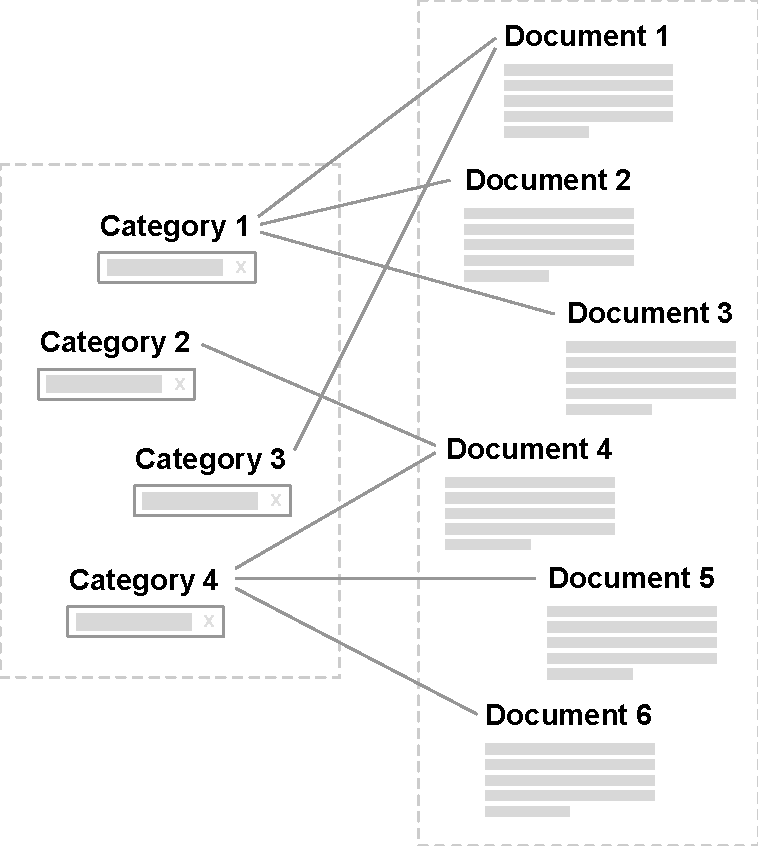
\includegraphics[width=0.5\textwidth]{img/bipartite-graph-text-classification}
  \end{center}
  \caption{Text classification visualized as a bipartite graph. Here the multi-label setting is shown where no additional constraints are enforced on the problem and hence each document can be assigned to multiple categories}
\label{fig:bipartite-graph-text-classification}
\end{wrapfigure}

Text classification, also known as text categorization, is the task of predicting a \emph{mapping} $\widetilde{\Phi} : \mathcal{D} \times \mathcal{C} \rightarrow \{True, False\}$ between a set of \emph{documents} $\mathcal{D}$ and a set of \emph{classes} or \emph{categories} $\mathcal{C}$ using a model function $\Phi : \mathcal{D} \times \mathcal{C} \rightarrow \{True, False \}$.
We thus aim to predict as well as possible the documents associated with each category or vice versa the categories that each document belongs into. The former is called \emph{category-pivoted} text classification whereas the latter is referred to as \emph{document-pivoted} text classification --- the setting that we shall focus on from here onwards.
The mapping $\widetilde{\Phi}$ can be represented as a bipartite graph between the set of documents $\mathcal{D}$ and the set of categories $\mathcal{C}$ as shown in Figure~\ref{fig:bipartite-graph-text-classification}. In this representation vertices in the graph represent a $True$ value in the mapping, indicating that the document and category are associated with each other, while missing vertices indicate that they are not which corresponds to a $False$ value in the mapping.

Categories $\mathcal{C}$ are given as symbolic labels and documents $\mathcal{D}$ as sequences of text with variable length. It is usually assumed that no additional information such as metadata or other \emph{exogenous knowledge} is available on neither labels nor documents.
As the survey on automatic text classification by~\cite{Sebastiani:2002aa} points, out a consequence of relying solely on \emph{endogenous knowledge}, especially the semantics of a text, is that there is no objective ground truth to this task in most settings since semantics are a \emph{subjective} notion: \textquote{This is exemplified by the phenomenon of inter-indexer inconsistency~\cite{Cleverdon:1984aa}: when two human experts decide whether to classify document $d_j$ under category $c_i$, they may disagree, and this in fact happens with relatively high frequency. A news article on Clinton attending Dizzy Gillespie’s funeral could be filed under Politics, or under Jazz, or under both, or even under neither, depending on the subjective judgment of the expert.}

Additional constraints can be imposed on the problem to adapt it for different application scenarios. Firstly text classification can be either framed as \emph{single-label} classification where each document is assigned to only one single category or \emph{multi-label} classification where an assignment to several categories or also no category is possible. The single-label case can be further separated into \emph{dichotomous} or \emph{binary} classification where the presence or absence of only a single class is predicted and \emph{multi-class} classification where one of multiple, mutually exclusive classes is predicted for each document.
Multi-class classification can thus be seen as multi-label classification with the additional constraint of classes being mutually exclusive.
If labels are assumed to be statistically independent multi-label classification can also be reformulated as $|\mathcal{C}|$ individual binary classification problems, potentially allowing much simpler modeling at the cost of introducing inductive bias through a strong assumption.

% In order to measure how successfully we are tackling the problem of text classification we need metrics that measure the effectiveness of our algorithm given a dataset. These will be discussed in Section~\ref{sub:Evaluation}.

\subsection{Problem Formalism: Multi-class Sentence Classification}
\label{subs:Problem Formalism: Multi-class Sentence Classification}

The prediction task in the scope of this thesis is \emph{Multi-class Sentence Classification} which shall be formulated as a special case of Text Classification defined above. Specifically the goal is to perform \emph{document-pivoted Multi-class Text Classification} where the documents $\mathcal{D}$ are the set of all sentences $S$ drawn \emph{uniformly and independently} at random from a set of job advertisements $\mathcal{J}$, and the classes $\mathcal{C}$ are set to be the following set of mutually exclusive labels $\mathcal{L} = \{ \text{benefits}, \text{candidate}, \text{company}, \text{job}, \text{nextsteps}, \text{other} \}$. We thus allow for no knowledge to be used regarding the origin of a sentence $s_i$, meaning that the prediction of each sentence is independent must assume the same prior information. The task can hence be expressed as predicting true label $l_i$ for a sentence $s_i$, i.e.\ finding the mapping $\widetilde{\Phi} : \mathcal{S} \rightarrow \mathcal{L}$.

\subsection{Dataset: Labelled Sentences from Job Advertisements}
\label{subs:Dataset: Labelled Sentences from Job Advertisements}

The performance of approaching the research problem will be evaluated using a dataset that was designed and created specifically for the purpose of this work. For detailed information on the process and design decisions involved please refer to Section~\ref{sub:Definition Phase: Framing the Problem} (\nameref{sub:Definition Phase: Framing the Problem}). Here the key characteristics of the data will be shown.

\begin{figure}[h]
  % From http://localhost:8888/notebooks/thesis/experiments/vector-space-models/Vector%20Space%20Models.ipynb#Setup
    \centering
    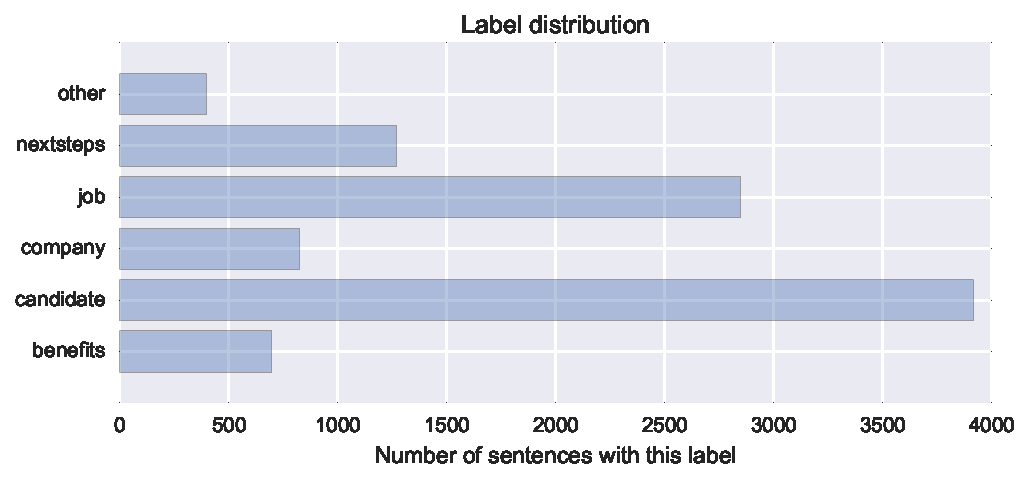
\includegraphics[width=\textwidth]{img/sentence-data-label-dist.pdf}
    \caption{Distribution of labels in sentence data}
\label{fig:sentence-data-label-dist}
\end{figure}

The data from this set stems from job advertisements created by companies using the \gls{Sanoma}'s service \gls{Oikotie Tyopaikat} in Finland. Each job posting contains many fields of associated metadata such as the title of the job posting, the time of creation and many more. Of these only the \emph{job description} was chosen as a basis for this task since --- as pointed out previously in Section~\ref{subs:Context: Definition of Text Classification} --- the task of interest was pure text classification without exogenous knowledge with the motivation to better understand unstructured data such as the job description which does not follow a specific format. The dataset was collected using the \gls{Crowdsourcing} service \gls{CrowdFlower} as described in detail in Section~\ref{subs:Multi-class Sentence Classification}.

The resulting dataset consists of 9948 labelled sentences totaling to an amount of 121,119 words and 807,984 characters. To each sentence one of the following labels is assigned: \emph{benefits, candidate, company, job, nextsteps, other}. Table~\ref{tab:Labels, Description, Example Sentences} shows the meaning of each class and an example of a sentences associated with it. The resulting distribution of the labels is strongly skewed towards higher prevalence of several labels as shown in Figure~\ref{fig:sentence-data-label-dist}.

\begin{table}[h]
  \begin{center}
  \begin{tabularx}{\textwidth}{l | X | X}
    \toprule
    Label & Description & Example Sentence \\
    \midrule
    benefits & \textbf{Benefits}: Rewards, opportunities, reasons to apply, \ldots & And we like to think we’ll give you an enjoyable and inspiring place to spend your working day. \\
    candidate & \textbf{Candidate requirements}: Requirements, skills, experience, education, personality, \ldots & To succeed in this position it is essential to have strong experience of at least 5 years in international business development and/or international B2B sales and marketing. \\
    company & \textbf{Company information}: Company name, story, mission, structure, market share, \ldots & Progman is software house specialising in the development of software for Building Services. \\
    job & \textbf{Job description}: Role, responsibilities, location of work, type of employment, \ldots & Your main objective is to maximize Core Fleet, Dealer B2B, municipality and governmental orders and sales for PC and LCV range to local Fleets and businesses within defined geographical area. \\
    nextsteps & \textbf{Next steps}: Call to action, application procedure, contact, further information, \ldots & 040 75 67 316, Mon-Fri 10-14, or peas@temp-team.fi. \\
    other & \textbf{Other}: Does not fit into the above categories & URS’ \\
    \bottomrule
  \end{tabularx}
  \caption{Labels used for the task with their description that was given for the participants labelling the data and a sentence example for each label.}
\label{tab:Labels, Description, Example Sentences}
\end{center}
\end{table}

% Reader will not know MCC yet
\glsreset{MCC}

\subsection{Performance Metric: Matthews Correlation Coefficient}
\label{sub:Performance Metric: Matthews Correlation Coefficient}

As a metric for predictive performance \gls{MCC} was chosen which is described in detail in Section~\ref{sub:Evaluation Metrics} along with other performance metrics. This metric is used relatively rarely used in the machine learning literature as opposed to e.g.\ the F1 score that is common in the \gls{IR} literature where ignoring True Negatives can be tolerated. As an example we do not generally care if a search engine predicts correctly all the billions of website we don't want to see for a search query as long as it retrieves enough relevant ones.
However, with the dataset at hand a metric was needed that measures prediction reliably and without bias even in case of a strongly skewed distribution of labels. Stratified sampling from the dataset to achieve a balanced distribution was not an option since the dataset was too small. Thus \gls{MCC} was selected which fulfills these criteria and additionally is easy to interpret: It is a correlation score between -1 and 1, denoting anti-correlation and correlation respectively.
